\documentclass[tikz,border=2pt]{standalone}
\usepackage{amsmath}
\usepackage{pgfplots}
\pgfplotsset{compat=1.18}
\usetikzlibrary{arrows.meta}
\begin{document}
% Triangle V={x1+x2<=3, x1>=0, x2>=0} with a1=(1,1), a2=(-1,0), a3=(0,-1). Normal cones drawn at each point:
% p1=(3,0): I={1,3}, Cone({a1,a3}); p2=(1,2): I={1}, half-line along a1; p3=(1,1): I empty, {0}.
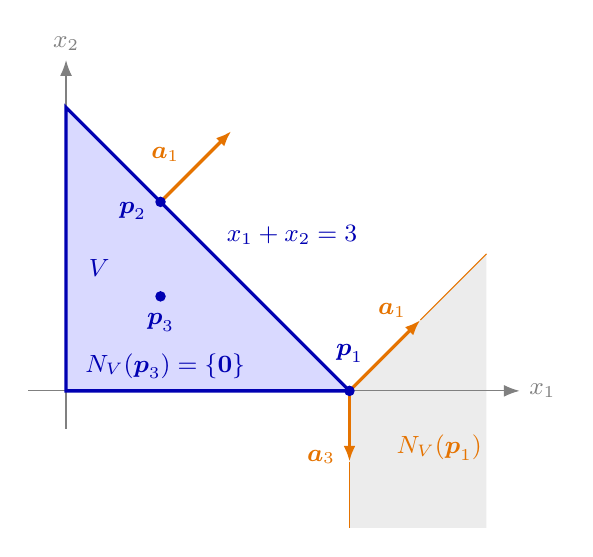
\begin{tikzpicture}[font=\small, >={Latex[length=2mm]}, x=1.2cm, y=1.2cm]
  \fill[gray!15] (3,0) -- (3,-1.45) -- (4.45,-1.45) -- (4.45,1.45) -- cycle;
  \fill[blue!15] (0,0) -- (3,0) -- (0,3) -- cycle;
  \draw[gray, ->] (-0.4,0) -- (4.8,0) node[anchor=west] {$x_1$};
  \draw[gray, ->] (0,-0.4) -- (0,3.5) node[anchor=south] {$x_2$};
  \draw[blue!70!black, very thick] (0,0) -- (3,0) -- (0,3) -- cycle;
  \node[blue!70!black, anchor=south west] at (1.6,1.45) {$x_1+x_2=3$};
  \node[blue!70!black] at (0.35,1.3) {$V$};
  % p1: two binding rows
  \draw[orange!90!black, very thick, ->] (3,0) -- (3.75,0.75);
  \draw[orange!90!black, very thick, ->] (3,0) -- (3,-0.75);
  \draw[orange!90!black, thin] (3.75,0.75) -- (4.45,1.45);
  \draw[orange!90!black, thin] (3,-0.75) -- (3,-1.45);
  \node[orange!90!black, anchor=east] at (3.7,0.85) {$\boldsymbol{a}_1$};
  \node[orange!90!black, anchor=east] at (2.95,-0.7) {$\boldsymbol{a}_3$};
  \node[orange!90!black] at (3.95,-0.6) {$N_V(\boldsymbol{p}_1)$};
  \fill[blue!70!black] (3,0) circle (1.9pt);
  \node[blue!70!black, anchor=south] at (3,0.2) {$\boldsymbol{p}_1$};
  % p2: one binding row
  \draw[orange!90!black, very thick, ->] (1,2) -- (1.75,2.75);
  \node[orange!90!black, anchor=east] at (1.3,2.5) {$\boldsymbol{a}_1$};
  \fill[blue!70!black] (1,2) circle (1.9pt);
  \node[blue!70!black, anchor=east] at (0.95,1.9) {$\boldsymbol{p}_2$};
  % p3: interior point
  \fill[blue!70!black] (1,1) circle (1.9pt);
  \node[blue!70!black, anchor=north] at (1,0.92) {$\boldsymbol{p}_3$};
  \node[blue!70!black, anchor=north] at (1.05,0.5) {$N_V(\boldsymbol{p}_3)=\{\boldsymbol{0}\}$};
\end{tikzpicture}
\end{document}
